% This file was created with tikzplotlib v0.10.1.
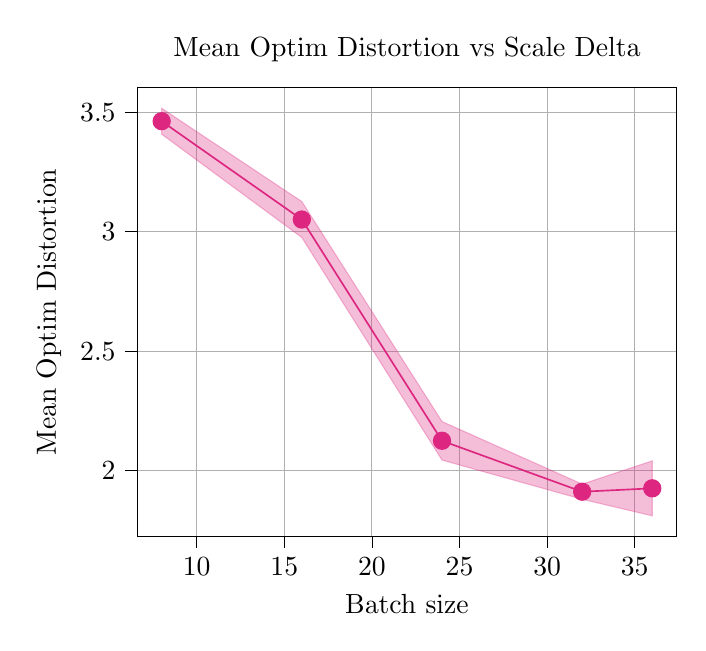
\begin{tikzpicture}

\definecolor{darkgray176}{RGB}{176,176,176}
\definecolor{mediumvioletred22038127}{RGB}{220,38,127}

\begin{axis}[
tick align=outside,
tick pos=left,
title={Mean Optim Distortion vs Scale Delta},
x grid style={darkgray176},
xlabel={Batch size},
xmajorgrids,
xmin=6.6, xmax=37.4,
xtick style={color=black},
y grid style={darkgray176},
ylabel={Mean Optim Distortion},
ymajorgrids,
ymin=1.72517988100207, ymax=3.60257640114329,
ytick style={color=black}
]
\path [draw=mediumvioletred22038127, fill=mediumvioletred22038127, opacity=0.3]
(axis cs:8,3.51724019568232)
--(axis cs:8,3.40865747697088)
--(axis cs:16,2.97595422473396)
--(axis cs:24,2.04398519332256)
--(axis cs:32,1.8797260404173)
--(axis cs:36,1.81051608646303)
--(axis cs:36,2.0406276007852)
--(axis cs:36,2.0406276007852)
--(axis cs:32,1.94310692829455)
--(axis cs:24,2.20534052937184)
--(axis cs:16,3.12652894959008)
--(axis cs:8,3.51724019568232)
--cycle;

\addplot [semithick, mediumvioletred22038127, mark=*, mark size=3, mark options={solid}]
table {%
8 3.4629488363266
16 3.05124158716202
24 2.1246628613472
32 1.91141648435593
36 1.92557184362411
};
\end{axis}

\end{tikzpicture}
